L'élaboration de ce cahier des charges s'est faite en deux phases. 
Dans un premier temps, j'ai participé à des réunions avec Grégory, Renaud et Sophie afin de démarrer le projet. 
Et dans un second temps, nous avons ajouté et adapté des fonctionnalités au fur et à mesure que le projet a avancé.

\paragraph{}
Altissia travaille selon les principes \Gls{g-agile} et plus précisément la méthodologie \Gls{g-scrum}.
Ces principes sont nés d'un constat sur les projets informatiques, la majorité échoue\cite{standish_standish_nodate} et la plupart du temps c'est parce que les besoins sont mal définis ou parce que la communication entre les parties prenantes est mauvaise (voir figure \ref{fig:why-projects-fails}).

\begin{figure}[ht]
    \centering
    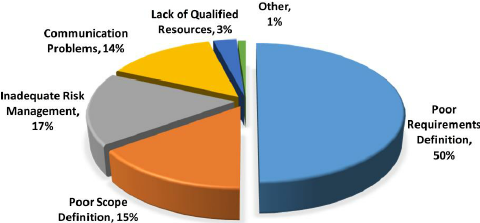
\includegraphics[scale=.8]{images/why-projects-fail.png}
    \caption{Role of Requirements in Software Project Failures. Source: ESI International Survey of 2000 Business Professionals, 2005.}
    \label{fig:why-projects-fails}
\end{figure}

\paragraph{}
Pour répondre à ces enjeux, le service informatique d'Altissia a adopté la méthode \Gls{g-scrum}.
Cela consiste à travailler de manière itérative, de régulièrement produire des résultats intermédiaires utilisables, d'impliquer les différents acteurs, d'obtenir leurs commentaires et d'adapter la direction du projet selon ceux-ci.

\paragraph{}
C'est donc pour cela que le cahier des charges n'est pas complet et définitif au début du projet, mais qu'il s'étoffe au fur et à mesure.
